\chapter{\ifproject%
\ifenglish Project Structure and Methodology\else โครงสร้างและขั้นตอนการทำงาน\fi
\else%
\ifenglish Project Structure\else โครงสร้างของโครงงาน\fi
\fi
}

ในบทนี้จะกล่าวถึงหลักการ, การนำทฤษฎีที่เกี่ยวข้องมาประยุกต์ใช้ และการออกแบบของระบบ

\makeatletter

% \renewcommand\section{\@startsection {section}{1}{\z@}%
%                                    {13.5ex \@plus -1ex \@minus -.2ex}%
%                                    {2.3ex \@plus.2ex}%
%                                    {\normalfont\large\bfseries}}

\makeatother
%\vspace{2ex}
% \titleformat{\section}{\normalfont\bfseries}{\thesection}{1em}{}
% \titlespacing*{\section}{0pt}{10ex}{0pt}

\section{การจัดเก็บข้อมูล}
โดยข้อมูลราคาหุ้นทุกตัวจะมีแหล่งที่มาจาก 2 ที่ก็คือ AlphaVantage และ Finnhub โดย AlphaVantage จะให้ข้อมูลย้อนหลังไป 2 ปี ส่วน Finnhub จะเอาไว้ใช้อัพเดท
ข้อมูลแบบ real-time ทุกๆ 1 ชม. เราใช้ MongoDB เป็น Database สำหรับจัดเก็บข้อมูลตลาดหุ้น และตัวชี้วัดทางเทคนิคที่เราต้องการใช้ เช่น RSI, MA เป็นต้น

ในตอนเริ่มตันนั้นเราดึงข้อมูลที่ต้องการมาจาก AlphaVantage ซึ่งก็คือข้อมูลตลาดหุ้นย้อนหลัง 2 ปีโดยใช้ API ของ AlphaVantage 
และเก็บข้อมูลลง MongoDB ด้วย Rust โดยมีการแปลงข้อมูลให้เป็นในรูปแบบข้อมูลตลาดของเราซึ่งก็จะประกอบด้วย
\begin{enumerate}
    \item ticker: ชื่อของหุ้นที่ทำการซื้อขาย เช่น AAPL/USD, IBM/USD
    \item open: เป็นราคาซื้อขายแรกที่เกิดขึ้นใน ช่วงเวลานั้นๆ
    \item close: เป็นราคาสุดท้ายที่เกิดขึ้นจากการซื้อขายสิ้นสุด ของช่วงเวลานั้นๆ
    \item high: การเคลื่อนไหวของราคาหุ้น ณ ระดับราคาสูงสุดในช่วงเวลานั้นๆ
    \item low: การเคลื่อนไหวของราคาหุ้น ณ ระดับราคาต่ำสุดในช่วงเวลานั้นๆ
    \item volume: ปริมาณการซื้อขายในช่วงเวลานั้นๆ
\end{enumerate}
จากนั้นในการ update ข้อมูลแบบ real-time เราจะใช้ MongoDB Scheduled Triggers ที่จะไปเรียกใช้ AWS Lambda ที่เราสร้างขึ้นมา โดยใน Lambda จะดึงข้อมูลจาก 
Finnhub มา update ซึ่งในการ update นี้ก็จะมีการ update ข้อมูลของตัวชี้วัดทางเทคนิคที่เราต้องการใช้ และ update ตัวชี้วัดทางเทคนิคของเราเองด้วย

\begin{figure}[ht]
    \centering
    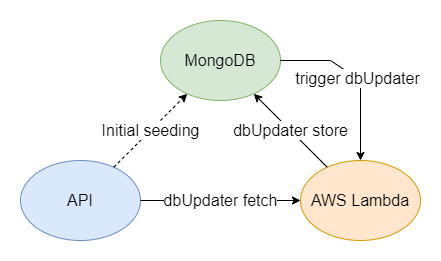
\includegraphics[scale=0.6]{images/db.png}
    \caption{โครงสร้างของการจัดเก็บข้อมูล โดนเส้นประคือทำครั้งเดียวในตอนแรกเริ่ม และเส้นทึบจะทำในทุกๆ ชม. โดยเป็นการเรียกใช้โปรแกรม dBUpdater ใน AWS Lambda}
    \label{fig:1}
\end{figure}